% Author: Izaak Neutelings (September 2020)
\documentclass[border=3pt,tikz]{standalone}
\usepackage{amsmath}
\usepackage{tikz}
\usepackage{physics}
\usetikzlibrary{intersections}
\usetikzlibrary{decorations.markings}
\usetikzlibrary{angles,quotes} % for pic
\usetikzlibrary{decorations.pathmorphing} % for decorate random steps
\tikzset{>=latex} % for LaTeX arrow head
\usepackage{xcolor}
\colorlet{xcol}{blue!70!black}
\colorlet{xcol'}{xcol!50!red!80!black}
\colorlet{veccol}{green!45!black}
\tikzstyle{vector}=[->,thick,veccol,line cap=round]
\tikzstyle{rvec}=[->,thick,xcol,line cap=round]


\begin{document}


% VECTOR breakdown on axis
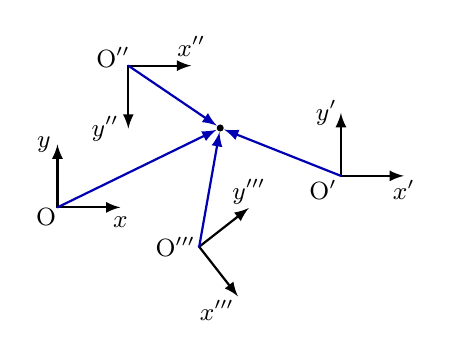
\begin{tikzpicture}
  \small
  \def\L{0.8}
  \def\R{2.3}
  \def\ang{26}
  \def\thet{-52}
  \coordinate (O) at (0,0);
  \coordinate (O1) at (3.6,0.4);
  \coordinate (O2) at (0.9,1.8);
  \coordinate (O3) at (1.8,-0.5);
  \coordinate (R) at (\ang:\R);
  \node[fill=black,circle,inner sep=0.9] (R') at (R) {};
  
  % O1
  \draw[<->,thick] (\L,0) node[below] {$x$} --
                   (O) node[below left=-3] {O} --
                   (0,\L) node[left=-1] {$y$};
  \draw[rvec] (O) -- (R');
  
  % O1
  \begin{scope}[shift={(O1)}]
    \draw[<->,thick] (\L,0) node[below=-2] {$x'$} --
                     (0,0) node[below left=-2] {O$'$} --
                     (0,\L) node[left=-2] {$y'$};
    \draw[rvec] (0,0) -- (R');
  \end{scope}
  
  % O2
  \begin{scope}[shift={(O2)}]
    \draw[<->,thick] (\L,0) node[above] {$x''$} --
                     (0,0) node[above left=-4] {O$''$} --
                     (0,-\L) node[left] {$y''$};
    \draw[rvec] (0,0) -- (R');
  \end{scope}
  
  % O3
  \begin{scope}[shift={(O3)}]
    \draw[<->,thick] (\thet:\L) node[below left=-2] {$x'''$} --
                     (0,0) node[left=-2] {O$'''$} --
                     (\thet+90:\L) node[above=-2] {$y'''$};
    \draw[rvec] (0,0) -- (R');
  \end{scope}
  
\end{tikzpicture}


% LAB & COM FRAMES
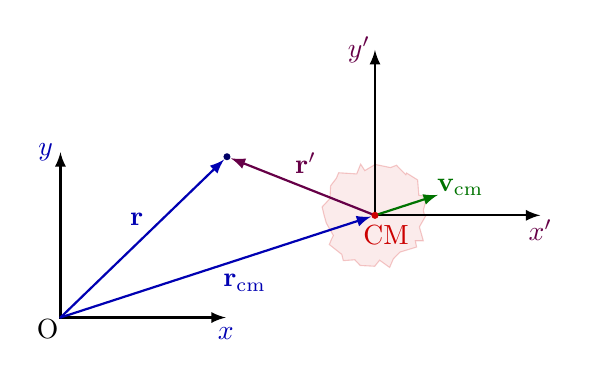
\begin{tikzpicture}
  \def\L{2.1}
  \def\ang{18} % angle of the CM velocity
  \coordinate (O) at (0,0);
  \coordinate (O') at (\ang:2.0*\L);
  \coordinate (R) at (44:1.4*\L);
  \node[fill=blue!40!black,circle,inner sep=0.9] (R') at (R) {};
  
  % LAB
  \draw[<->,thick] (\L,0) node[below,xcol] {$x$} --
                   (O) node[below left=-3] {O} --
                   (0,\L) node[left=-1,xcol] {$y$};
  \draw[rvec] (O) -- (R') node[midway,left=2,above=1] {$\vb{r}$}; %$(\vb{r})_\mathrm{lab}$
  
  % COM
  \draw[red!80!black,fill=red!80!black!40,opacity=0.2,
        decorate,decoration={random steps,segment length=3pt,amplitude=2pt}]
    (O') circle(0.3*\L);
  \draw[<->,thick] (O')++(\L,0) node[below=-2,xcol'] {$x'$} --++
                   (-\L,0) node[red!80!black,right=4,below] {CM} --++
                   (0,\L) node[left=-2,xcol'] {$y'$};
  \draw[rvec,xcol'] (O') -- (R') node[midway,right=1,above=1] {$\vb{r}'$}; %(\vb{r})_\mathrm{cm}
  \draw[vector] (O') --++ (\ang:0.4*\L) node[above right=-4] {$\vb{v}_\mathrm{cm}$}; %(\vb{v}_\mathrm{cm})_\mathrm{lab}
  \node[fill=red!80!black,circle,inner sep=0.9] (CM) at (O') {};
  \draw[rvec] (O) -- (CM) node[midway,below right=-1] {$\vb{r}_\mathrm{cm}$}; %(\vb{r}_\mathrm{cm})_\mathrm{lab}
  
\end{tikzpicture}




\end{document}